\documentclass{standalone}
\usepackage{tikz}
\usetikzlibrary{patterns, positioning}
\usepackage[sfdefault]{ClearSans} %% option 'sfdefault' activates Clear Sans as the default text font
\usepackage[T1]{fontenc}

\begin{document}
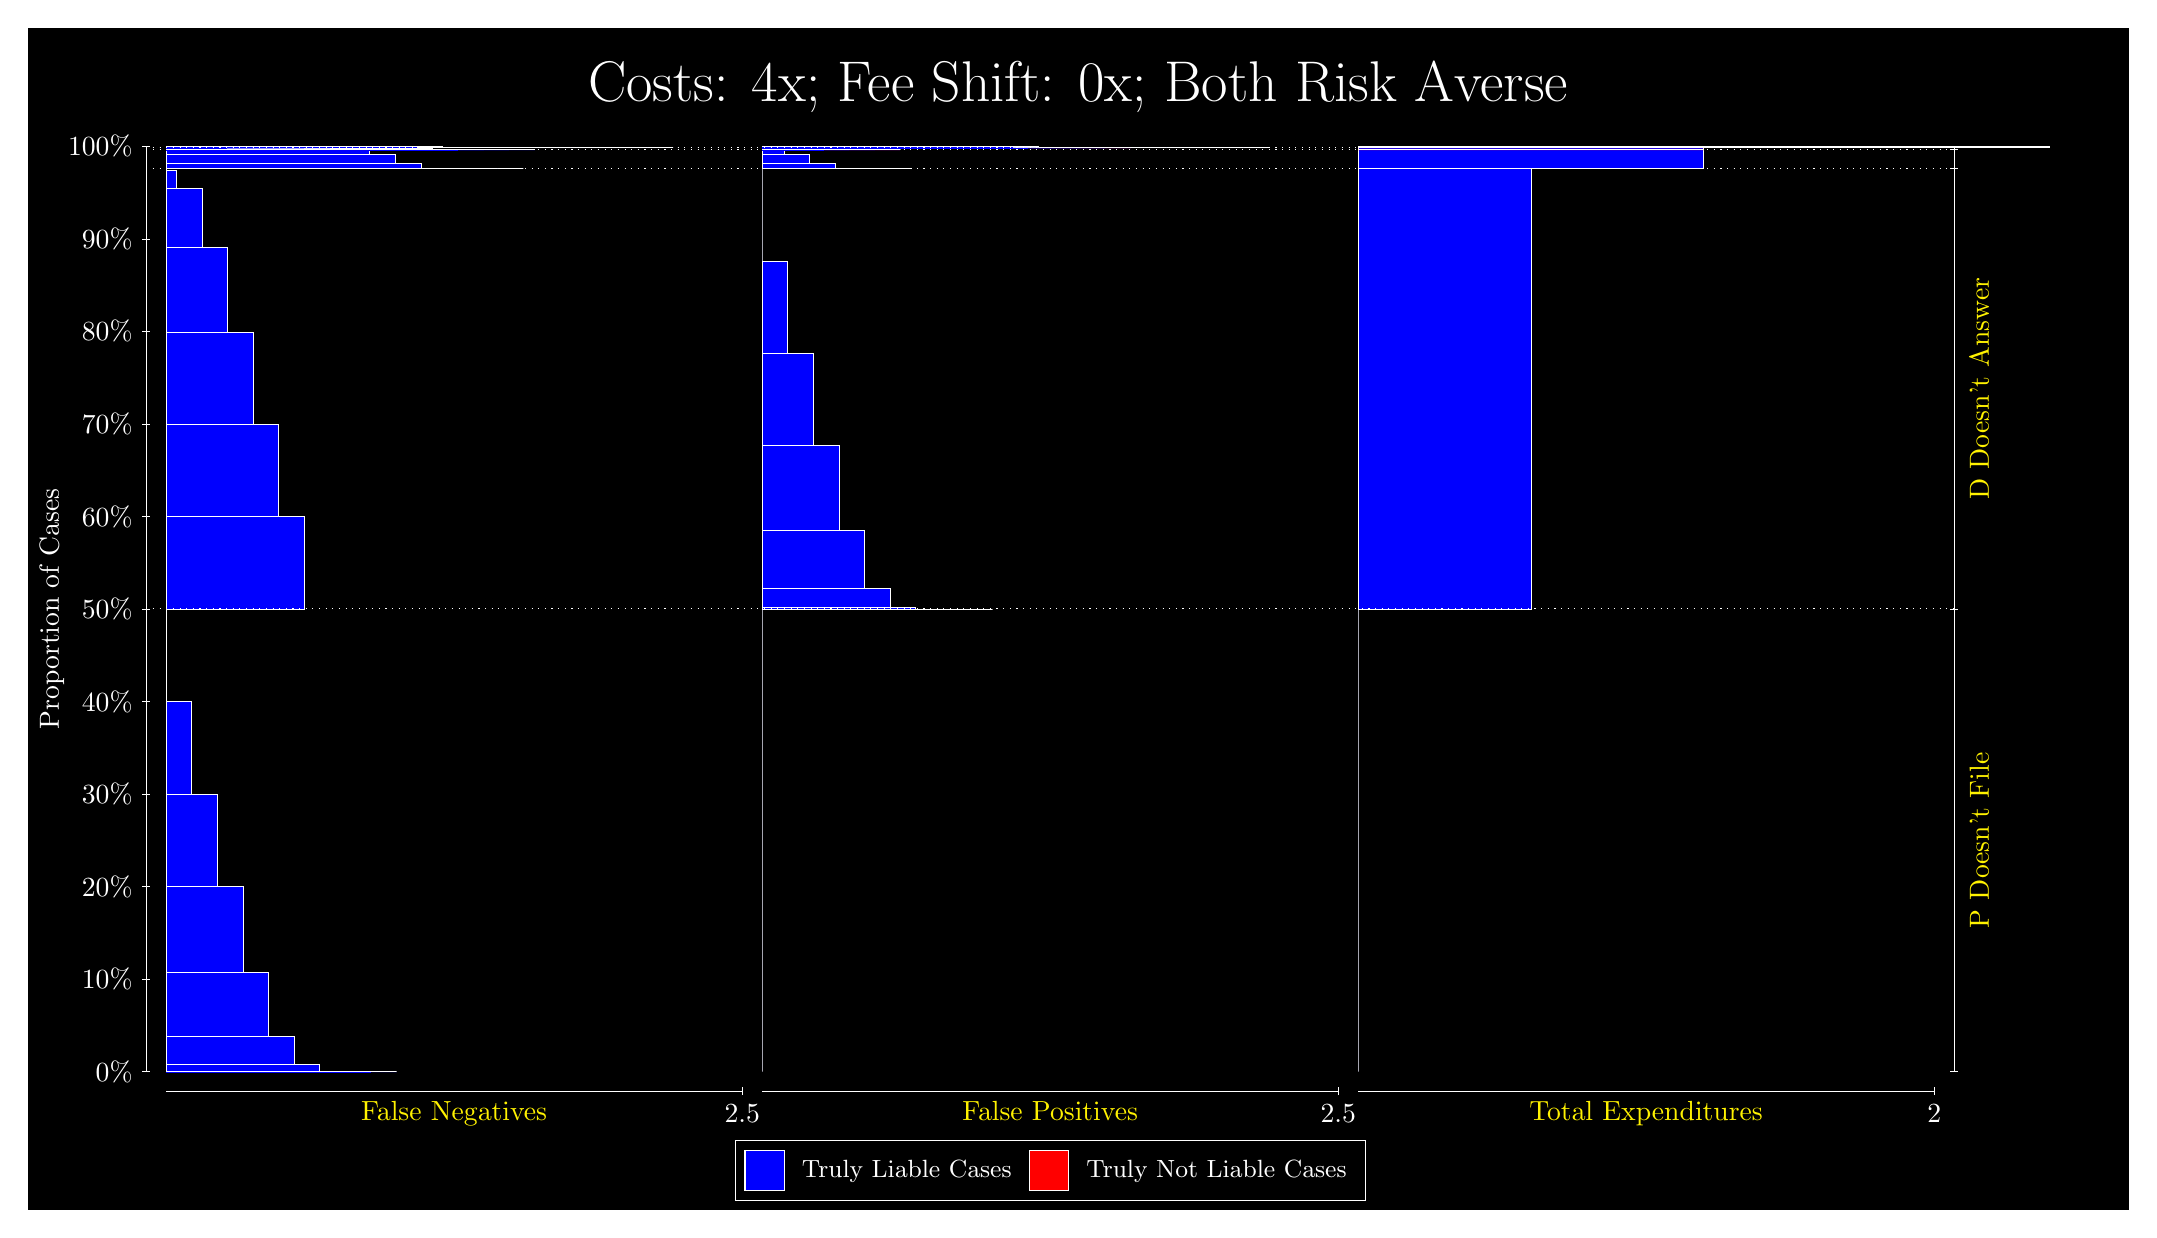
\begin{tikzpicture}
\draw[fill=black] (0,0) rectangle (26.667,15);
\draw[text=white] (0,13.5) rectangle (26.667,15) node[midway] {\huge Costs: 4x; Fee Shift: 0x; Both Risk Averse};
\draw[white, very thin] (1.5,1.75) -- (1.5,13.5);
\node[rotate=90, text=white, anchor=center] at (0.3, 7.625) {Proportion of Cases};
\draw[white, very thin] (1.45,1.75) -- (1.55,1.75);
\node[text=white, anchor=east] at (1.45, 1.75) {0\%};
\draw[white, very thin] (1.45,2.925) -- (1.55,2.925);
\node[text=white, anchor=east] at (1.45, 2.925) {10\%};
\draw[white, very thin] (1.45,4.1) -- (1.55,4.1);
\node[text=white, anchor=east] at (1.45, 4.1) {20\%};
\draw[white, very thin] (1.45,5.275) -- (1.55,5.275);
\node[text=white, anchor=east] at (1.45, 5.275) {30\%};
\draw[white, very thin] (1.45,6.45) -- (1.55,6.45);
\node[text=white, anchor=east] at (1.45, 6.45) {40\%};
\draw[white, very thin] (1.45,7.625) -- (1.55,7.625);
\node[text=white, anchor=east] at (1.45, 7.625) {50\%};
\draw[white, very thin] (1.45,8.8) -- (1.55,8.8);
\node[text=white, anchor=east] at (1.45, 8.8) {60\%};
\draw[white, very thin] (1.45,9.975) -- (1.55,9.975);
\node[text=white, anchor=east] at (1.45, 9.975) {70\%};
\draw[white, very thin] (1.45,11.15) -- (1.55,11.15);
\node[text=white, anchor=east] at (1.45, 11.15) {80\%};
\draw[white, very thin] (1.45,12.325) -- (1.55,12.325);
\node[text=white, anchor=east] at (1.45, 12.325) {90\%};
\draw[white, very thin] (1.45,13.5) -- (1.55,13.5);
\node[text=white, anchor=east] at (1.45, 13.5) {100\%};

\draw[white, very thin] (24.457,1.75) -- (24.457,13.5);
\draw[white, very thin] (24.407,1.75) -- (24.507,1.75);
\node[anchor=west] at (24.407, 1.75) {};
\draw[white, very thin] (24.407,7.625) -- (24.507,7.625);
\node[anchor=west] at (24.407, 7.625) {};
\draw[white, very thin] (24.407,13.219) -- (24.507,13.219);
\node[anchor=west] at (24.407, 13.219) {};
\draw[white, very thin] (24.407,13.457) -- (24.507,13.457);
\node[anchor=west] at (24.407, 13.457) {};
\draw[white, very thin] (24.407,13.482) -- (24.507,13.482);
\node[anchor=west] at (24.407, 13.482) {};
\draw[white, very thin] (24.407,13.49) -- (24.507,13.49);
\node[anchor=west] at (24.407, 13.49) {};
\draw[white, very thin] (24.407,13.5) -- (24.507,13.5);
\node[anchor=west] at (24.407, 13.5) {};

\draw[white, very thin, fill=blue] (1.75,1.75) rectangle (4.6775,1.75);
\draw[white, very thin, fill=blue] (1.75,1.75) rectangle (4.3523,1.7503);
\draw[white, very thin, fill=blue] (1.75,1.7503) rectangle (4.027,1.7576);
\draw[white, very thin, fill=blue] (1.75,1.7576) rectangle (3.7017,1.8362);
\draw[white, very thin, fill=blue] (1.75,1.8362) rectangle (3.3764,2.1987);
\draw[white, very thin, fill=blue] (1.75,2.1987) rectangle (3.0511,3.0112);
\draw[white, very thin, fill=blue] (1.75,3.0112) rectangle (2.7258,4.1076);
\draw[white, very thin, fill=blue] (1.75,4.1076) rectangle (2.4006,5.2753);
\draw[white, very thin, fill=blue] (1.75,5.2753) rectangle (2.0753,6.45);
\draw[white, very thin, fill=red] (1.75,6.45) rectangle (1.75,6.45);
\draw[white, very thin, fill=blue] (1.75,6.45) rectangle (1.75,7.625);
\draw[white, very thin, fill=blue] (1.75,7.625) rectangle (3.5065,8.8);
\draw[white, very thin, fill=blue] (1.75,8.8) rectangle (3.1812,9.9747);
\draw[white, very thin, fill=blue] (1.75,9.9747) rectangle (2.856,11.141);
\draw[white, very thin, fill=blue] (1.75,11.141) rectangle (2.5307,12.224);
\draw[white, very thin, fill=blue] (1.75,12.224) rectangle (2.2054,12.961);
\draw[white, very thin, fill=blue] (1.75,12.961) rectangle (1.8801,13.196);
\draw[white, very thin, fill=red] (1.75,13.196) rectangle (1.75,13.196);
\draw[white, very thin, fill=blue] (1.75,13.196) rectangle (1.75,13.219);
\draw[white, very thin, fill=blue] (1.75,13.219) rectangle (6.2877,13.219);
\draw[white, very thin, fill=blue] (1.75,13.219) rectangle (5.9624,13.219);
\draw[white, very thin, fill=blue] (1.75,13.219) rectangle (5.6371,13.219);
\draw[white, very thin, fill=blue] (1.75,13.219) rectangle (5.3118,13.226);
\draw[white, very thin, fill=blue] (1.75,13.226) rectangle (4.9866,13.282);
\draw[white, very thin, fill=blue] (1.75,13.282) rectangle (4.6613,13.396);
\draw[white, very thin, fill=blue] (1.75,13.396) rectangle (4.336,13.45);
\draw[white, very thin, fill=blue] (1.75,13.45) rectangle (4.0107,13.457);
\draw[white, very thin, fill=blue] (1.75,13.457) rectangle (3.6854,13.457);
\draw[white, very thin, fill=blue] (1.75,13.457) rectangle (3.3602,13.457);
\draw[white, very thin, fill=red] (1.75,13.457) rectangle (1.75,13.457);
\draw[white, very thin, fill=blue] (1.75,13.457) rectangle (6.4341,13.457);
\draw[white, very thin, fill=blue] (1.75,13.457) rectangle (6.1088,13.457);
\draw[white, very thin, fill=blue] (1.75,13.457) rectangle (5.7835,13.457);
\draw[white, very thin, fill=blue] (1.75,13.457) rectangle (5.4582,13.459);
\draw[white, very thin, fill=blue] (1.75,13.459) rectangle (5.1329,13.469);
\draw[white, very thin, fill=blue] (1.75,13.469) rectangle (4.8077,13.479);
\draw[white, very thin, fill=blue] (1.75,13.479) rectangle (4.4824,13.481);
\draw[white, very thin, fill=blue] (1.75,13.481) rectangle (4.1571,13.482);
\draw[white, very thin, fill=blue] (1.75,13.482) rectangle (3.8318,13.482);
\draw[white, very thin, fill=blue] (1.75,13.482) rectangle (3.5065,13.482);
\draw[white, very thin, fill=red] (1.75,13.482) rectangle (1.75,13.482);
\draw[white, very thin, fill=blue] (1.75,13.482) rectangle (3.5065,13.482);
\draw[white, very thin, fill=blue] (1.75,13.482) rectangle (3.1812,13.482);
\draw[white, very thin, fill=blue] (1.75,13.482) rectangle (2.856,13.482);
\draw[white, very thin, fill=blue] (1.75,13.482) rectangle (2.5307,13.485);
\draw[white, very thin, fill=blue] (1.75,13.485) rectangle (2.2054,13.489);
\draw[white, very thin, fill=blue] (1.75,13.489) rectangle (1.8801,13.49);
\draw[white, very thin, fill=red] (1.75,13.49) rectangle (1.75,13.49);
\draw[white, very thin, fill=blue] (1.75,13.49) rectangle (1.75,13.49);
\draw[white, very thin, fill=blue] (1.75,13.49) rectangle (8.1906,13.49);
\draw[white, very thin, fill=blue] (1.75,13.49) rectangle (7.8653,13.49);
\draw[white, very thin, fill=blue] (1.75,13.49) rectangle (7.54,13.49);
\draw[white, very thin, fill=blue] (1.75,13.49) rectangle (7.54,13.49);
\draw[white, very thin, fill=blue] (1.75,13.49) rectangle (7.2148,13.49);
\draw[white, very thin, fill=blue] (1.75,13.49) rectangle (6.8895,13.49);
\draw[white, very thin, fill=blue] (1.75,13.49) rectangle (6.5642,13.49);
\draw[white, very thin, fill=blue] (1.75,13.49) rectangle (6.2389,13.49);
\draw[white, very thin, fill=blue] (1.75,13.49) rectangle (5.9136,13.491);
\draw[white, very thin, fill=blue] (1.75,13.491) rectangle (5.9136,13.491);
\draw[white, very thin, fill=blue] (1.75,13.491) rectangle (5.5883,13.493);
\draw[white, very thin, fill=blue] (1.75,13.493) rectangle (5.5883,13.494);
\draw[white, very thin, fill=blue] (1.75,13.494) rectangle (5.2631,13.496);
\draw[white, very thin, fill=blue] (1.75,13.496) rectangle (4.9378,13.497);
\draw[white, very thin, fill=blue] (1.75,13.497) rectangle (4.9378,13.498);
\draw[white, very thin, fill=blue] (1.75,13.498) rectangle (4.6125,13.498);
\draw[white, very thin, fill=blue] (1.75,13.498) rectangle (4.6125,13.5);
\draw[white, very thin, fill=blue] (1.75,13.5) rectangle (4.6125,13.5);
\draw[white, very thin, fill=blue] (1.75,13.5) rectangle (4.2872,13.5);
\draw[white, very thin, fill=blue] (1.75,13.5) rectangle (4.2872,13.5);
\draw[white, very thin, fill=blue] (1.75,13.5) rectangle (3.9619,13.5);
\draw[white, very thin, fill=blue] (1.75,13.5) rectangle (3.6366,13.5);
\draw[white, very thin, fill=blue] (1.75,13.5) rectangle (3.3114,13.5);
\draw[white, very thin, fill=blue] (1.75,13.5) rectangle (3.3114,13.5);
\draw[white, very thin, fill=blue] (1.75,13.5) rectangle (2.9861,13.5);
\draw[white, very thin, fill=blue] (1.75,13.5) rectangle (2.9861,13.5);
\draw[white, very thin, fill=blue] (1.75,13.5) rectangle (2.6608,13.5);
\draw[white, very thin, fill=blue] (1.75,13.5) rectangle (2.6608,13.5);
\draw[white, very thin, fill=blue] (1.75,13.5) rectangle (2.3355,13.5);
\draw[white, very thin, fill=red] (1.75,13.5) rectangle (1.75,13.5);
\draw[white, very thin, fill=red] (9.3189,1.75) rectangle (9.3189,1.75);
\draw[white, very thin, fill=blue] (9.3189,1.75) rectangle (9.3189,7.625);
\draw[white, very thin, fill=red] (9.3189,7.625) rectangle (12.246,7.625);
\draw[white, very thin, fill=blue] (9.3189,7.625) rectangle (12.246,7.625);
\draw[white, very thin, fill=blue] (9.3189,7.625) rectangle (11.921,7.625);
\draw[white, very thin, fill=blue] (9.3189,7.625) rectangle (11.596,7.6254);
\draw[white, very thin, fill=blue] (9.3189,7.6254) rectangle (11.271,7.6476);
\draw[white, very thin, fill=blue] (9.3189,7.6476) rectangle (10.945,7.8832);
\draw[white, very thin, fill=blue] (9.3189,7.8832) rectangle (10.62,8.6199);
\draw[white, very thin, fill=blue] (9.3189,8.6199) rectangle (10.295,9.7024);
\draw[white, very thin, fill=blue] (9.3189,9.7024) rectangle (9.9694,10.869);
\draw[white, very thin, fill=blue] (9.3189,10.869) rectangle (9.6442,12.044);
\draw[white, very thin, fill=blue] (9.3189,12.044) rectangle (9.3189,13.219);
\draw[white, very thin, fill=red] (9.3189,13.219) rectangle (11.222,13.219);
\draw[white, very thin, fill=blue] (9.3189,13.219) rectangle (11.222,13.219);
\draw[white, very thin, fill=blue] (9.3189,13.219) rectangle (10.896,13.219);
\draw[white, very thin, fill=blue] (9.3189,13.219) rectangle (10.571,13.226);
\draw[white, very thin, fill=blue] (9.3189,13.226) rectangle (10.246,13.28);
\draw[white, very thin, fill=blue] (9.3189,13.28) rectangle (9.9206,13.393);
\draw[white, very thin, fill=blue] (9.3189,13.393) rectangle (9.5954,13.45);
\draw[white, very thin, fill=blue] (9.3189,13.45) rectangle (9.3189,13.457);
\draw[white, very thin, fill=red] (9.3189,13.457) rectangle (11.075,13.457);
\draw[white, very thin, fill=blue] (9.3189,13.457) rectangle (11.075,13.457);
\draw[white, very thin, fill=blue] (9.3189,13.457) rectangle (10.75,13.457);
\draw[white, very thin, fill=blue] (9.3189,13.457) rectangle (10.425,13.457);
\draw[white, very thin, fill=blue] (9.3189,13.457) rectangle (10.1,13.459);
\draw[white, very thin, fill=blue] (9.3189,13.459) rectangle (9.7743,13.47);
\draw[white, very thin, fill=blue] (9.3189,13.47) rectangle (9.449,13.48);
\draw[white, very thin, fill=blue] (9.3189,13.48) rectangle (9.3189,13.482);
\draw[white, very thin, fill=red] (9.3189,13.482) rectangle (14.003,13.482);
\draw[white, very thin, fill=blue] (9.3189,13.482) rectangle (14.003,13.482);
\draw[white, very thin, fill=blue] (9.3189,13.482) rectangle (13.678,13.482);
\draw[white, very thin, fill=blue] (9.3189,13.482) rectangle (13.352,13.482);
\draw[white, very thin, fill=blue] (9.3189,13.482) rectangle (13.027,13.482);
\draw[white, very thin, fill=blue] (9.3189,13.482) rectangle (12.702,13.483);
\draw[white, very thin, fill=blue] (9.3189,13.483) rectangle (12.377,13.486);
\draw[white, very thin, fill=blue] (9.3189,13.486) rectangle (12.051,13.489);
\draw[white, very thin, fill=blue] (9.3189,13.489) rectangle (11.726,13.49);
\draw[white, very thin, fill=blue] (9.3189,13.49) rectangle (11.401,13.49);
\draw[white, very thin, fill=blue] (9.3189,13.49) rectangle (11.075,13.49);
\draw[white, very thin, fill=red] (9.3189,13.49) rectangle (15.759,13.49);
\draw[white, very thin, fill=blue] (9.3189,13.49) rectangle (15.759,13.49);
\draw[white, very thin, fill=blue] (9.3189,13.49) rectangle (15.434,13.49);
\draw[white, very thin, fill=red] (9.3189,13.49) rectangle (15.434,13.49);
\draw[white, very thin, fill=blue] (9.3189,13.49) rectangle (15.434,13.49);
\draw[white, very thin, fill=red] (9.3189,13.49) rectangle (15.109,13.49);
\draw[white, very thin, fill=blue] (9.3189,13.49) rectangle (15.109,13.49);
\draw[white, very thin, fill=blue] (9.3189,13.49) rectangle (15.109,13.49);
\draw[white, very thin, fill=blue] (9.3189,13.49) rectangle (14.784,13.49);
\draw[white, very thin, fill=red] (9.3189,13.49) rectangle (14.784,13.49);
\draw[white, very thin, fill=blue] (9.3189,13.49) rectangle (14.784,13.49);
\draw[white, very thin, fill=blue] (9.3189,13.49) rectangle (14.784,13.49);
\draw[white, very thin, fill=blue] (9.3189,13.49) rectangle (14.458,13.49);
\draw[white, very thin, fill=red] (9.3189,13.49) rectangle (14.458,13.49);
\draw[white, very thin, fill=blue] (9.3189,13.49) rectangle (14.458,13.49);
\draw[white, very thin, fill=blue] (9.3189,13.49) rectangle (14.458,13.49);
\draw[white, very thin, fill=blue] (9.3189,13.49) rectangle (14.133,13.49);
\draw[white, very thin, fill=red] (9.3189,13.49) rectangle (14.133,13.49);
\draw[white, very thin, fill=blue] (9.3189,13.49) rectangle (14.133,13.49);
\draw[white, very thin, fill=blue] (9.3189,13.49) rectangle (14.133,13.49);
\draw[white, very thin, fill=blue] (9.3189,13.49) rectangle (13.808,13.49);
\draw[white, very thin, fill=blue] (9.3189,13.49) rectangle (13.808,13.49);
\draw[white, very thin, fill=red] (9.3189,13.49) rectangle (13.808,13.49);
\draw[white, very thin, fill=blue] (9.3189,13.49) rectangle (13.808,13.49);
\draw[white, very thin, fill=blue] (9.3189,13.49) rectangle (13.808,13.49);
\draw[white, very thin, fill=blue] (9.3189,13.49) rectangle (13.482,13.49);
\draw[white, very thin, fill=blue] (9.3189,13.49) rectangle (13.482,13.491);
\draw[white, very thin, fill=red] (9.3189,13.491) rectangle (13.482,13.491);
\draw[white, very thin, fill=blue] (9.3189,13.491) rectangle (13.482,13.491);
\draw[white, very thin, fill=blue] (9.3189,13.491) rectangle (13.157,13.492);
\draw[white, very thin, fill=red] (9.3189,13.492) rectangle (13.157,13.492);
\draw[white, very thin, fill=blue] (9.3189,13.492) rectangle (13.157,13.494);
\draw[white, very thin, fill=blue] (9.3189,13.494) rectangle (13.157,13.494);
\draw[white, very thin, fill=blue] (9.3189,13.494) rectangle (12.832,13.494);
\draw[white, very thin, fill=red] (9.3189,13.494) rectangle (12.832,13.494);
\draw[white, very thin, fill=blue] (9.3189,13.494) rectangle (12.832,13.496);
\draw[white, very thin, fill=blue] (9.3189,13.496) rectangle (12.832,13.496);
\draw[white, very thin, fill=blue] (9.3189,13.496) rectangle (12.507,13.497);
\draw[white, very thin, fill=blue] (9.3189,13.497) rectangle (12.507,13.498);
\draw[white, very thin, fill=blue] (9.3189,13.498) rectangle (12.507,13.498);
\draw[white, very thin, fill=blue] (9.3189,13.498) rectangle (12.181,13.498);
\draw[white, very thin, fill=blue] (9.3189,13.498) rectangle (12.181,13.499);
\draw[white, very thin, fill=blue] (9.3189,13.499) rectangle (12.181,13.5);
\draw[white, very thin, fill=blue] (9.3189,13.5) rectangle (11.856,13.5);
\draw[white, very thin, fill=blue] (9.3189,13.5) rectangle (11.856,13.5);
\draw[white, very thin, fill=blue] (9.3189,13.5) rectangle (11.856,13.5);
\draw[white, very thin, fill=blue] (9.3189,13.5) rectangle (11.531,13.5);
\draw[white, very thin, fill=blue] (9.3189,13.5) rectangle (11.531,13.5);
\draw[white, very thin, fill=blue] (9.3189,13.5) rectangle (11.206,13.5);
\draw[white, very thin, fill=blue] (9.3189,13.5) rectangle (11.206,13.5);
\draw[white, very thin, fill=blue] (9.3189,13.5) rectangle (11.206,13.5);
\draw[white, very thin, fill=blue] (9.3189,13.5) rectangle (10.88,13.5);
\draw[white, very thin, fill=blue] (9.3189,13.5) rectangle (10.88,13.5);
\draw[white, very thin, fill=blue] (9.3189,13.5) rectangle (10.555,13.5);
\draw[white, very thin, fill=blue] (9.3189,13.5) rectangle (10.555,13.5);
\draw[white, very thin, fill=blue] (9.3189,13.5) rectangle (10.555,13.5);
\draw[white, very thin, fill=blue] (9.3189,13.5) rectangle (10.23,13.5);
\draw[white, very thin, fill=blue] (9.3189,13.5) rectangle (9.9044,13.5);
\draw[white, very thin, fill=red] (16.888,1.75) rectangle (16.888,1.75);
\draw[white, very thin, fill=blue] (16.888,1.75) rectangle (16.888,7.625);
\draw[white, very thin, fill=red] (16.888,7.625) rectangle (19.083,7.625);
\draw[white, very thin, fill=blue] (16.888,7.625) rectangle (19.083,13.219);
\draw[white, very thin, fill=red] (16.888,13.219) rectangle (21.279,13.219);
\draw[white, very thin, fill=blue] (16.888,13.219) rectangle (21.279,13.457);
\draw[white, very thin, fill=red] (16.888,13.457) rectangle (21.279,13.457);
\draw[white, very thin, fill=blue] (16.888,13.457) rectangle (21.279,13.482);
\draw[white, very thin, fill=red] (16.888,13.482) rectangle (21.279,13.482);
\draw[white, very thin, fill=blue] (16.888,13.482) rectangle (21.279,13.49);
\draw[white, very thin, fill=red] (16.888,13.49) rectangle (25.67,13.49);
\draw[white, very thin, fill=blue] (16.888,13.49) rectangle (25.67,13.49);
\draw[white, very thin, fill=red] (16.888,13.49) rectangle (25.67,13.49);
\draw[white, very thin, fill=blue] (16.888,13.49) rectangle (25.67,13.499);
\draw[white, very thin, fill=red] (16.888,13.499) rectangle (25.67,13.499);
\draw[white, very thin, fill=blue] (16.888,13.499) rectangle (25.67,13.5);
\draw[white, dotted] (1.5,7.625) -- (24.457,7.625);
\draw[white, dotted] (1.5,13.219) -- (24.457,13.219);
\draw[white, dotted] (1.5,13.457) -- (24.457,13.457);
\draw[white, dotted] (1.5,13.482) -- (24.457,13.482);
\draw[white, dotted] (1.5,13.49) -- (24.457,13.49);
\draw[white, very thin] (1.75,1.5) -- (9.0689,1.5);
\node[text=yellow, anchor=north] at (5.4094, 1.5) {False Negatives};
\draw[white, very thin] (9.0689,1.45) -- (9.0689,1.55);
\node[text=white, anchor=north] at (9.0689, 1.45) {2.5};

\draw[white, very thin] (9.3189,1.5) -- (16.638,1.5);
\node[text=yellow, anchor=north] at (12.978, 1.5) {False Positives};
\draw[white, very thin] (16.638,1.45) -- (16.638,1.55);
\node[text=white, anchor=north] at (16.638, 1.45) {2.5};

\draw[white, very thin] (16.888,1.5) -- (24.207,1.5);
\node[text=yellow, anchor=north] at (20.547, 1.5) {Total Expenditures};
\draw[white, very thin] (24.207,1.45) -- (24.207,1.55);
\node[text=white, anchor=north] at (24.207, 1.45) {2};

\node[text=yellow, centered, rotate=90] at (24.777, 4.6875) {P Doesn't File};
\node[text=yellow, centered, rotate=90] at (24.777, 10.422) {D Doesn't Answer};





\draw (12.978300999999998,1.5) node[draw=none] (baseCoordinate) {};
\begin{scope}[align=center]
        \matrix[scale=0.5, draw=white, below=0.5cm of baseCoordinate, nodes={draw}, column sep=0.1cm]{
            \node[rectangle, draw, minimum width=0.5cm, minimum height=0.5cm, fill=blue] {}; &
            \node[draw=none, font=\small, text=white] (B) {Truly Liable Cases}; &
            \node[rectangle, draw, minimum width=0.5cm, minimum height=0.5cm, fill=red] {}; &
            \node[draw=none, font=\small, text=white] (B) {Truly Not Liable Cases}; \\
            };
\end{scope}

\end{tikzpicture}
\end{document}